\documentclass[11pt,ngerman,a4paper]{article}
%Gummi|061|=)
\usepackage{amsmath}
\usepackage{a4wide}
\usepackage{amsthm}
\usepackage{amsbsy}
\usepackage{amssymb}
\usepackage{inputenc}
\usepackage{rotating} 
\usepackage{graphicx}
\usepackage{paralist}
\usepackage{selinput}
\SelectInputMappings{%
adieresis={ä},
germandbls={ß},
}
\title{\textbf{Versuch V354: Gedämpfte und erzwungene Schwingungen}}
\author{Martin Bieker\\
		Julian Surmann\\
		\\
		Durchgef\"{u}hrt am 19.12.2013\\
		Tu Dortmund}
\date{}
\usepackage{graphicx}
\begin{document}
\renewcommand\tablename{Tabelle}
\renewcommand\figurename{Abbildung}
\maketitle
\thispagestyle{empty}
\newpage
\clearpage
\setcounter{page}{1}


\section{Einleitung}
In diesem Versuch sollen gedämpfte und erzwungene Schwingungen am Beispiel des elektrischen Schwingkreises untersucht werden. Dieses System besteht aus zwei Energiespeichern, einem Kondensator und einer Spule. Zwischen diesen Energiespeichern pendelt die Energie hin und her. Unter (theoretischen) idealen Bedingungen ist diese Schwingung ungedämpft. In dem zu untersuchenden Versuchsaufbau ist jedoch ein Widerstand eingebaut, so wird eine gedämpfte Schwingung beobachtet.
\section{Theorie}
Bei dem Versuchsaufbau handelt es sich um einen gedämpften harmonischen Oszillator. Mit Hilfe der Kirchhoffschen Regeln und dem Induktionsgesetz kann die Differentialgleichung des hier verwendeten Oszillators hergeleitet werden. Sie lautet
\begin{equation}
\label{DGL}
\frac{d^2 I}{d t^2} + \frac{R}{L} \frac{d I}{d t} + \frac{I}{LC} = 0.
\end{equation}
Um diese Differentialgleichung zu lösen, ist eine Fallunterscheidung von Nöten.\newline
Für den Schwingfall lautet die Lösung
\begin{equation}
\label{LSG1}
I(t) = A_0 e^{-2 \pi \mu t} cos (2 \pi \nu t + \eta).
\end{equation}
Für den aperiodischen Grenzfall lautet sie
\begin{equation}
\label{LSG2}
I(t) = A e^{- \frac{t}{\sqrt{LC}}}.
\end{equation}
\section{Aufbau und Durchf\"{u}hrung}
Die Schaltung des elektrischen Schwingkreises ist fest aufgebaut. Es stehen mehrere Widerstände zur Verfügung, davon ein Potentiometer. Ein Signalgenerator wird benutzt, um das System anzuregen. Für die Messungen wird ein digitales Speicheroszilloskop verwendet.
\subsection{Untersuchung der Zeitabhängigkeit der Amplitude}
Um die Zeitabhängigkeit der Amplitude zu untersuchen, wird der elektrische Schwingkreis mit einzelnen Nadelimpulsen angeregt. Das System beginnt zu Schwingen. Mit dem hochohmigen Tastkopf wird die Spannung des Kondensators auf die Y-Ablenkung des Speicheroszilloskops gegeben. Der entstehende Graph soll für die Auswertung gespeichert werden. Bei diesem Versuchsteil ist der kleinere Widerstand zu verwenden. Der Versuchsaufbau dieses Versuchsteiles ist in Abbildung \ref{S1} zu sehen.
\begin{figure}[h]
\centering
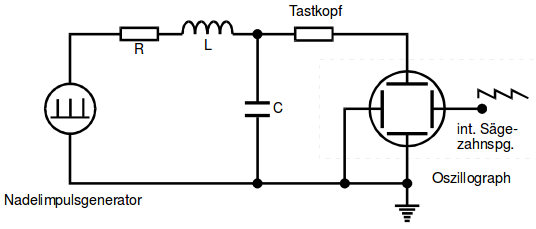
\includegraphics[scale=0.7]{Aufbau1.png}
\caption{Schaltung zur Messung der Zeitabhängigkeit der Amplitude}
\label{S1}
\end{figure}
\subsection{Bestimmung des Dämpfungswiderstandes bei aperiodischem Grenzfall}
In diesem Versuchsteil soll der Dämpfungswiderstand $R_{ap}$, bei dem die Schwingung den aperiodische Grenzfall annimmt, ermittelt werden. Dazu wird in der Schaltung aus Abbildung \ref{S1} lediglich der konstante Widerstand gegen das Potentiometer ausgetauscht. Das Potentiometer wird nun in maximale Stellung gebracht, der Kriechfall sollte zu erkennen sein. Nun wird der Widerstand solange verändert, bis man zwischen dem Kriech- und Schwingfall den aperiodischen Grenzfall möglichst gut angenähert hat.
\subsection{Messung der Frequenzabhängigkeit der Kondensatorspannung}
In dieser Messung wird die Frequenz des Erregers verändert und dabei die Auswirkung auf die maximale Kondensatorspannung untersucht. Da der verwendete Tastkopf auf einen spezifischen Frequenzgang besitzt, muss auch die Erregerspannung gemessen werden. In der Auswertung wird dann der Quotient $U_C / U_{Er}$ ermittelt.
Dieser Versuchsteil wird mit Hilfe der Schaltung in Abbildung \ref{S2} durchgeführt. Dabei soll der größere konstante Widerstand verwendet werden.
\begin{figure}[h]
\centering
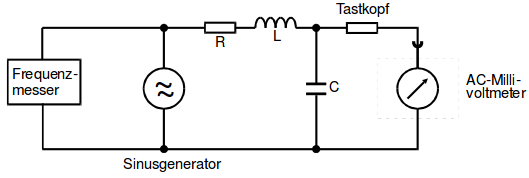
\includegraphics[scale=0.7]{Aufbau2.png}
\caption{Schaltung zur Messung der Frequenzabhängigkeit von $U_C$}
\label{S2}
\end{figure}
\subsection{Bestimmung der Frequenzabhängigkeit der Phase}
Zur Bestimmung der Phasendifferenz zwischen der Generator- und der Kondensatorspannung werden beide Spannungen auf die Y-Achse des Speicheroszilloskops gelegt. Bei einer Phasenverschiebung mit $\varphi \neq 0$ sind die beiden Kurven so gut zu erkennen. Die Phasenverschiebung wird dann mit Hilfe der Nulldurchgänge der Schwingungen ermittelt. Dafür müssen die beiden Sinuskurven allerdings symmetrisch zur x-Achse liegen. Die verwendete Schaltung ist der Abbildung \ref{S3} zu entnehmen.
\begin{figure}[h]
\centering
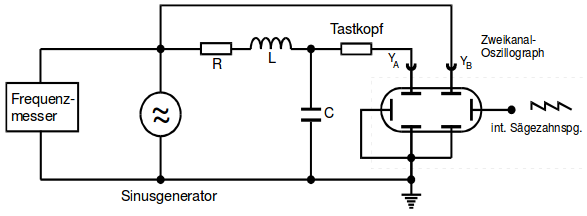
\includegraphics[scale=0.7]{Aufbau3.png}
\caption{Schaltung zur Bestimmung der Frequenzabhängigkeit der Phase}
\label{S3}
\end{figure}



\section{Auswertung}
\subsection{Bestimmung der Zeitkonstante}
Abbildung \ref{abb1} zeigt den Verlauf der Spannung $U_C$ zwischen den Platten des Kondensators unmittelbar nach dem Abschalten der Aufladespannung. 

==========

In der Tabelle \ref{mtab1} finden sich die lokalen Extrema des Spannungsverlaufs. Abbildung \ref{mabb2} ist eine halb-logarithmische Darstellung dieser Werte. In diesem Diagramm liegen die Messpunkte entlang der Geraden
\begin{equation}
ln(\frac{U_C}{V}) = -\frac{1}{RC}\cdot t + ln(U_0).
\end{equation}
Durch eine lineare Regression ergeben sich folgende Werte:
\begin{itemize}
\item $\frac{1}{RC} = ....\,\frac{1}{s}$
\end{itemize}
\subsection{Bestimmung des Grenzwiderstands}
\subsection{Bestimmung der Resonanzfrequenz}
\subsection{Bestimmung der Phasenverschiebung}



\section{Diskussion}
Hier kommt die Diskussion hin.
\section{Literatur- und Abbildungsverzeichnis}
Hier befindet sich das Literatur- und Abbildungsverzeichnis.
\section{Anhang}
Hier stehen die im Anhang angefügten Dokumente.
\end{document}
